\documentclass[12pt]{article}
%Gummi|065|=)
\usepackage{amsmath, amsfonts, amssymb}
\usepackage[margin=0.5in]{geometry}
\usepackage{xcolor}
%\usepackage{graphicx}
%\usepackage{graphicx}
\newcommand{\off}[1]{}
\DeclareMathSizes{20}{30}{21}{18}

\newcommand{\myhrule}{}

\newcommand{\two }{\sqrt[3]{2}}
\newcommand{\four}{\sqrt[3]{4}}

\newcommand{\dash}{
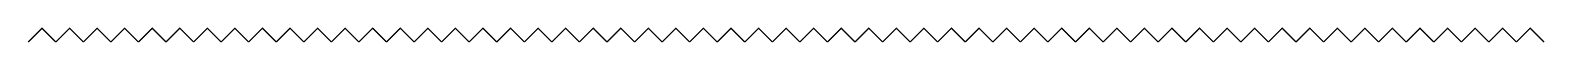
\begin{tikzpicture}[scale=0.35]
\foreach \x in {1,...,55}{
	\draw (\x,-0.25)--(\x+0.5,0.25)--(\x+1,-0.25);
}
\end{tikzpicture}
}

\usepackage{tikz}

\title{\textbf{ Examples: Pell Equation}}
\author{John D Mangual}
\date{}
\begin{document}

\fontfamily{qag}\selectfont \fontsize{25}{30}\selectfont

\maketitle

\noindent \textbf{Ex \#1} Consider $1, \sqrt[3]{2}, \sqrt[3]{4}$ generating $\mathbb{Z}[\sqrt[3]{2}]$.  What happens if we multiply by $\sqrt[3]{2}$ ?

$$
\begin{array}{ccccrcrcr}
\two &\cdot& 1 &=& a &+& b \,\two &+& c \,\four \\
\two &\cdot& \two &=& 2c &+& a \,\two &+& b \,\four \\
\two &\cdot& \four &=& 2b &+& 2c \,\two &+& a \,\four 
\end{array}
$$
Here is the equation for units (vectors of size 1)
$$ \det \left[
\begin{array}{ccc}
a & 2c & 2c \\
b & a & 2c \\
c & b & a
\end{array}
 \right] = a^3 + 2b^3 + 4c^3 - 6abc = 1 $$
 This is very much like the Pell equation. \\ \\
 \textbf{Ex \# 2} In the quadratic case, $K = \mathbb{Q}[\sqrt{2}]$.  The equation is:
 $$ \det \left[\begin{array}{cc} a & 2b \\ b & a\end{array} \right] = a^2 - 2b^2 = 1$$
 and remember the continued fraction of the square root of two
 $$ \sqrt{2} = 1 + \frac{1}{2 + \frac{1}{2 + \dots } }  = [1; 2,2,2,\dots ] = [1; \overline{2}]$$
Does there exixt an analogous shorthand for Ex \#1\\ \\
Can we solve $\sqrt[3]{2} = \dots $ in a similar way?

\newpage

\fontfamily{qag}\selectfont \fontsize{12}{10}\selectfont


\begin{thebibliography}{}

\item ...


\end{thebibliography}



\end{document}